\documentclass{beamer}
\usepackage{tikz}
\usepackage{ifthen}
\usepackage{fp}
\usetikzlibrary{shapes.geometric}
%Information to be included in the title page:
\title{Multi-Port Memory with Bidirectional Ports for FPGAs Using XOR and LVT Methods}
\author{Kevin Townsend}
\date{2026}

\begin{document}

\begin{frame}
\frametitle{Multi-Port Memory with Bidirectional Ports for FPGAs Using XOR and LVT Methods}
  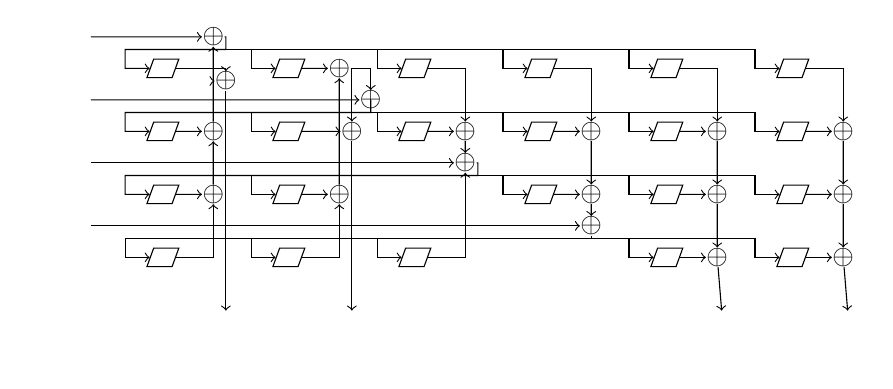
\begin{tikzpicture}[scale=0.8]
  \foreach \x in {0,1,2,3,4,5} {
    \foreach \y in {0,1,2,3} {
      \ifthenelse{\(\x = 2 \AND \y = 1\) \OR \(\x = 3 \AND \y = 0\)}{}{
        \node (r\x\y)[trapezium, trapezium left angle=70, trapezium right angle=110, draw] at (2*\x, \y){};
      }
    }
  }
  \foreach \x in {0,1,4,5} {
    \node (bport\x)[] at (2*\x+1, -1){};
  }
  \foreach \y in {0,1,2,3} {
    \node (lport\y)[] at (-1.3, 3.5-\y){};
  }
  \node [rotate=90] at (-2, .8){};
  \node [rotate=90] at (-2, 2.8){};
  \node [] at (1.5, -1.5){};
  \node [] at (9.5, -1.5){};
  \node(x50)[inner sep=0pt] at (10.8, 0){$\oplus$};
  \node(x51)[inner sep=0pt] at (10.8, 1){$\oplus$};
  \node(x52)[inner sep=0pt] at (10.8, 2){$\oplus$};
  \draw[->] (r50) -- (x50);
  \draw[->] (r51) -- (x51);
  \draw[->] (r52) -- (x52);
  \draw[->] (r53) -| (x52);
  \draw[->] (x52) -- (x51);
  \draw[->] (x51) -- (x50);
  \draw[->] (x50) -- (bport5.130);
  \node(x40)[inner sep=0pt] at (8.8, 0){$\oplus$};
  \node(x41)[inner sep=0pt] at (8.8, 1){$\oplus$};
  \node(x42)[inner sep=0pt] at (8.8, 2){$\oplus$};
  \draw[->] (r40) -- (x40);
  \draw[->] (r41) -- (x41);
  \draw[->] (r42) -- (x42);
  \draw[->] (r43) -| (x42);
  \draw[->] (x42) -- (x41);
  \draw[->] (x41) -- (x40);
  \draw[->] (x40) -- (bport4.130);
  \node(x31)[inner sep=0pt] at (6.8, 1){$\oplus$};
  \node(x32)[inner sep=0pt] at (6.8, 2){$\oplus$};
  \node(x30)[inner sep=0pt] at (6.8, .5){$\oplus$};
  \draw[->] (r31) -- (x31);
  \draw[->] (r32) -- (x32);
  \draw[->] (r33) -| (x32);
  \draw[->] (x32) -- (x31);
  \draw[->] (x31) -- (x30);
  %PORT3 connections.
  \draw[->] (lport3) -- (x30);
  \draw[->] (x30) |- (-.6,.3) |- (r00);
  \draw[->] (1.4,.3) |- (r10);
  \draw[->] (3.4,.3) |- (r20);
  \draw[->] (6.8, .3) -| (7.4,0) -- (r40);
  \draw[->] (7.4, .3) -| (9.4,0) -- (r50);
  %PORT2 XORs
  \node(x22)[inner sep=0pt] at (4.8, 2){$\oplus$};
  \node(x21)[inner sep=0pt] at (4.8, 1.5){$\oplus$};
  %PORT2 connections
  \draw[->] (lport2) -- (x21);
  \draw[->] (r23) -| (x22);
  \draw[->] (r22) -- (x22);
  \draw[->] (x22) -- (x21);
  \draw[->] (r20) -| (x21);
  \draw[->] (x21) -| (5,1.3) -| (-.6,1) -- (r01);
  \draw[->] (1.4,1.3) |- (r11);
  \draw[->] (5,1.3) -- (9.4, 1.3) |- (r51);
  \draw[->] (7.4, 1.3) |- (r41);
  \draw[->] (5.4, 1.3) |- (r31);
  %draw xor of full ports
  %PORT1
  \node(x11)[inner sep=0pt] at (2.8, 1){$\oplus$};
  \node(x12)[inner sep=0pt] at (3.3, 2.5){$\oplus$};
  \node(x12b)[inner sep=0pt] at (3, 2){$\oplus$};
  \node(x13)[inner sep=0pt] at (2.8, 3){$\oplus$};
  \draw[->] (r10) -| (x11);
  \draw[->] (r11) -- (x11);
  \draw[->] (lport1) -- (x12);
  \draw[->] (x11) -- (x13);
  \draw[->] (r13) -- (x13);
  \draw[->] (x13) -| (x12);
  \draw[->] (r12) -- (x12b);
  \draw[->] (x12) -| (3.3, 2.3) -| (-.6,2) -- (r02);
  \draw[->] (1.4,2.3) |- (r12);
  \draw[->] (3.3, 2.3) -- (9.4, 2.3) |- (r52);
  \draw[->] (3.4, 2.3) |- (r22);
  \draw[->] (5.4, 2.3) |- (r32);
  \draw[->] (7.4, 2.3) |- (r42);
  \draw[->] (x13) -| (x12b);
  \draw[->] (x12b) -- (bport1);
  %PORT0
  \node(x01)[inner sep=0pt] at (0.8, 1){$\oplus$};
  \node(x02)[inner sep=0pt] at (0.8, 2){$\oplus$};
  \node(x03)[inner sep=0pt] at (0.8, 3.5){$\oplus$};
  \node(x03b)[inner sep=0pt] at (1.0, 2.8){$\oplus$};
  \draw[->] (r00) -| (x01);
  \draw[->] (r01) -- (x01);
  \draw[->] (x01) -- (x02);
  \draw[->] (x02) -- (x03);
  \draw[->] (lport0) -- (x03);
  \draw[->] (x03) -| (1, 3.3) -| (-.6,3) -- (r03);
  \draw[->] (1, 3.3) -- (9.4, 3.3) |- (r53);
  \draw[->] (1.4, 3.3) |- (r13);
  \draw[->] (3.4, 3.3) |- (r23);
  \draw[->] (5.4, 3.3) |- (r33);
  \draw[->] (7.4, 3.3) |- (r43);
  \draw[->] (.8, 2.8) -- (x03b);
  \draw[->] (r02) -- (x02);
  \draw[->] (r03) -| (x03b);
  \draw[->] (x03b) -- (bport0);
  \end{tikzpicture}
\end{frame}

\end{document}
